%-%-%-%--%-%-%-%-%-%--%-%-%--%-%
% Author  : Tiago Chedraoui Silva
% License : GNU GPL v.3
% Title   : Mapa mental
% Tags    : mindmap, layers
%-%-%-%-%-%-%-%-%-%--%-%-%-%-%-%
\documentclass{article}
\usepackage{tikz,times}
\usepackage[paperwidth=55cm,paperheight=42cm,left=1cm,top=1cm]{geometry}
\usetikzlibrary{mindmap,backgrounds}

\pagestyle{empty}
\begin{document}
\centering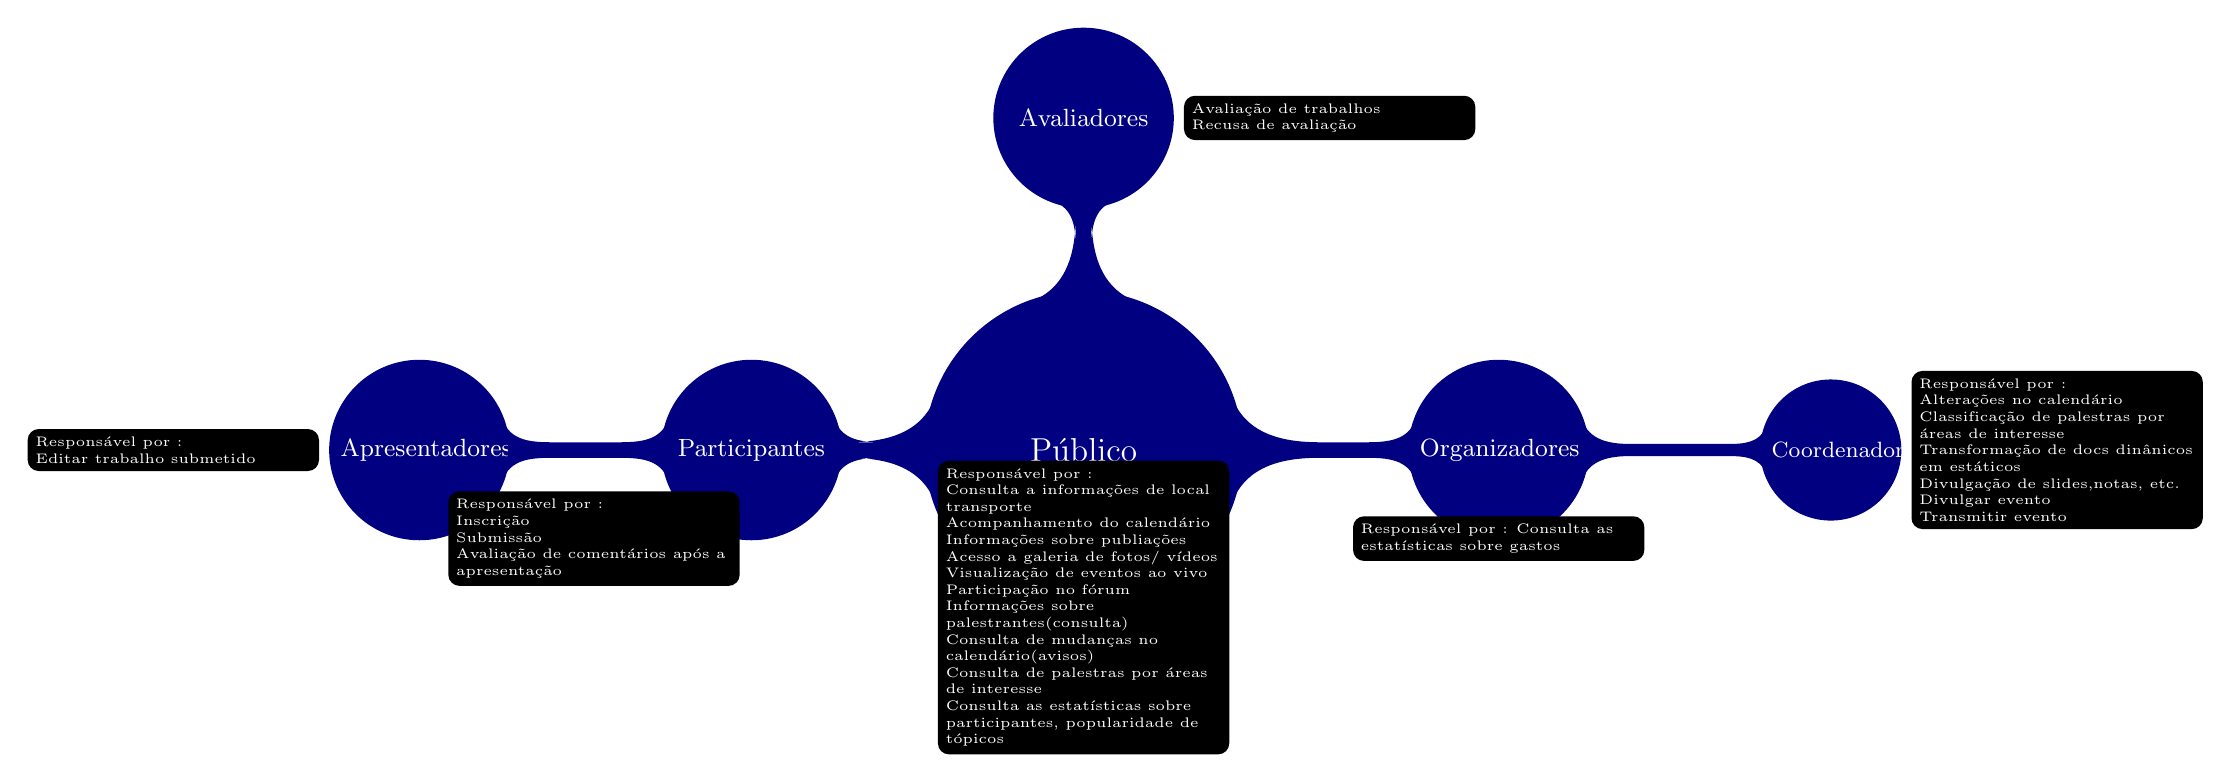
\begin{tikzpicture}[mindmap,
  level 1 concept/.append style={level distance=130,sibling angle=30},
  extra concept/.append style={color=blue!50,text=black},every annotation/.style={fill=black}]

  \begin{scope}[mindmap, concept color=blue!50!black, text=white,every annotation/.style={fill=black}]
    \node [concept](pub) at (0,-14.0)  {P\'ublico}
      child [grow=90, level distance=120] 
        {node [concept] (ava) {Avaliadores}}
    child [grow=0, level distance=150] 
        {node [concept] (org) {Organizadores}
	{ child [grow=0, level distance=120] 
	 {node [concept] (coo) {Coordenadores}}
	}   }
        child [grow=180, level distance=120] 
	{node [concept] (par) {Participantes}}
	{   child [grow=180, level distance=120] 
        {node [concept] (apr) {Apresentadores}} 
   
  };
     \node [annotation,right] at (ava.east)
      {Avalia\c{c}\~ao de trabalhos \\ Recusa de avalia\c{c}\~ao};
    \node [annotation,right] at (coo.east)
      {Respons\'avel por :\\Alterações no calend\'ario\\ Classifica\c{c}\~ao de palestras por \'areas de interesse \\ Transforma\c{c}\~ao de docs din\^anicos em est\'aticos\\Divulga\c{c}\~ao de slides,notas, etc. Divulgar evento\\ Transmitir evento};
    \node [annotation] at (org.south)
      {Respons\'avel por : Consulta as estat\'isticas sobre gastos};
    \node [annotation,left] at (apr.west)
      {Respons\'avel por :\\Editar trabalho submetido };

    \node [annotation] at (pub.south)
      {Respons\'avel por :\\Consulta a informa\c{c}\~oes de local \\ transporte \\ Acompanhamento do calend\'ario\\Informa\c{c}\~oes sobre publia\c{c}\~oes\\ Acesso a galeria de fotos/ v\'ideos\\ Visualiza\c{c}\~ao de eventos ao vivo\\Participa\c{c}\~ao no f\'orum\\ Informa\c{c}\~oes sobre palestrantes(consulta)\\Consulta de mudan\c{c}as no calend\'ario(avisos)\\Consulta de palestras por \'areas de interesse \\ Consulta as estat\'isticas sobre participantes, popularidade de t\'opicos };
   \node [annotation,left] at (par.south)
      {Respons\'avel por :\\Inscri\c{c}\~ao\\Submiss\~ao\\Avalia\c{c}\~ao de coment\'arios ap\'os a apresenta\c{c}\~ao };

   
\end{scope}


  % Connections of researchers to applied subfields

  \begin{pgfonlayer}{background}
   % \draw [circle connection bar]
  % \draw [concept connection ]
   %  (ac) edge (prc-ling)
   %  (c-tr) edge (uimp)
   %  (c-err) edge (org);
  
 \end{pgfonlayer}
\end{tikzpicture}

\end{document}
